
% !TEX program = pdflatex
% !TEX enableSynctex = true
% !BIB program = bibtex


\documentclass[12pt]{article}

\usepackage{setspace}
\usepackage{amsmath}
\usepackage{amsfonts}
\usepackage{graphicx}
\usepackage{float}
\addtolength{\oddsidemargin}{-.7in}
\addtolength{\evensidemargin}{-.7in}
\addtolength{\textwidth}{1.4in}
\usepackage{enumerate}
\onehalfspacing
\usepackage{geometry} % Required for customizing page layout

\usepackage{caption}
\usepackage{booktabs}

\usepackage{hyperref}
\hypersetup{
	pdfstartview = FitH,
	pdfauthor = {...},
	pdftitle = {...},
	pdfkeywords = {...; ...; ...; ...},
	colorlinks = true,
	linkcolor = blue,
	urlcolor = blue,
	citecolor = blue,
	linktocpage=true
}


\DeclareMathOperator{\E}{\mathbb{E}}
\DeclareMathOperator*{\argmax}{arg\,max}
\DeclareMathOperator*{\argmin}{arg\,min}

\begin{document}
\section*{Partial equilibrium model - firms' problem}
\subsection*{Ver 1 - PE model - Fixed q-s - 3 state variables}
Productivity process: two-state markov chain \vspace{3mm} \\
Labour policy: 
\begin{equation}
    n(k,\varepsilon_i) = \left( \dfrac{ \nu \varepsilon_i k^\alpha}{w} \right)^{\frac{1}{1-\nu}}
\end{equation}
Corresponding output: 
\begin{equation}
    y(k,\varepsilon_i) = \varepsilon_i k^{\alpha} \left( \dfrac{\nu \varepsilon_i k^\alpha}{w} \right)^{\frac{\nu}{1-\nu}}
\end{equation}
Corresponding profits: 
\begin{equation}
    \pi(k,\varepsilon_i) = (1-\nu) y(k,\varepsilon_i) - c
\end{equation}
External finance premium - just a parameter \vspace{2mm} \\
Value function:
\begin{equation}
     V(k,b, \varepsilon_i) = \max_{k',b'}  \left( \pi(k,\varepsilon_j)+(1-\delta)k - k' +  q^s b' -b  +
            \beta (1-P_\chi) \sum_{j=1}^{N_\varepsilon} g_{ij}  V(x',\varepsilon_j') \right)
\end{equation}
\noindent Here, the firm can directly choose $k'$ and $b'$, which makes coding the transition matrix easier, since you do not have to interpolate the Q-es. In the end you just have some very sparse matrices, since the model is almost deterministic. \vspace{3mm} \\
The shortcoming is you have 3 state variables and 2 action variables, which means that it is very hard to move past a grid size of 30. 

\newpage
\setcounter{equation}{0}


\subsection*{Ver 2 - Fixed Qs - cash on hand - two-state productivity}
Productivity process: two-state markov chain \vspace{3mm} \\
Labour policy: 
\begin{equation}
    n(k,\varepsilon_i) = \left( \dfrac{ \nu \varepsilon_i k^\alpha}{w} \right)^{\frac{1}{1-\nu}}
\end{equation}
Corresponding output: 
\begin{equation}
    y(k,\varepsilon_i) = \varepsilon_i k^{\alpha} \left( \dfrac{\nu \varepsilon_i k^\alpha}{w} \right)^{\frac{\nu}{1-\nu}}
\end{equation}
Corresponding profits: 
\begin{equation}
    \pi(k,\varepsilon_i) = (1-\nu) y(k,\varepsilon_i) - c
\end{equation}
Future cash on hand: 
\begin{equation}
   x' = \pi(k',\varepsilon_j')+(1-\delta)k'-b'
\end{equation}
External finance premium 
\begin{equation}
    q^s = 0.94
\end{equation}
Need an equity finance option. Otherwise there certain states are not associated to any feasible action. Here, I assume. This means that firms will sometimes have negative cash on hand. 
\begin{equation}
    d < 0 \implies d = 1.6d
\end{equation}
Value function:
\begin{equation}
     V(x,\varepsilon_i) = \max_{k',b'}  \left(x - k' +  q^s b' + 
            \beta  (1-P_\chi)  \sum_{j=1}^{N_\varepsilon} g_{ij} V(x',\varepsilon_j') \right)
\end{equation}
Adding cash on hand reduces the grid to 2 state and 2 action variables. This implies that you can do a much larger grid. However, you have to interpolate resulting x that follows from choices k' and b' to the grid, since x-here is the result. This could be a problem. Generally, results are well behaved in this case, although they are very mechanical. 


\begin{figure}[H]  % [h] indicates placing the image here
    \centering
    \caption{Ver2 - prod: 5, 8} \label{chart:CFLcdf}
    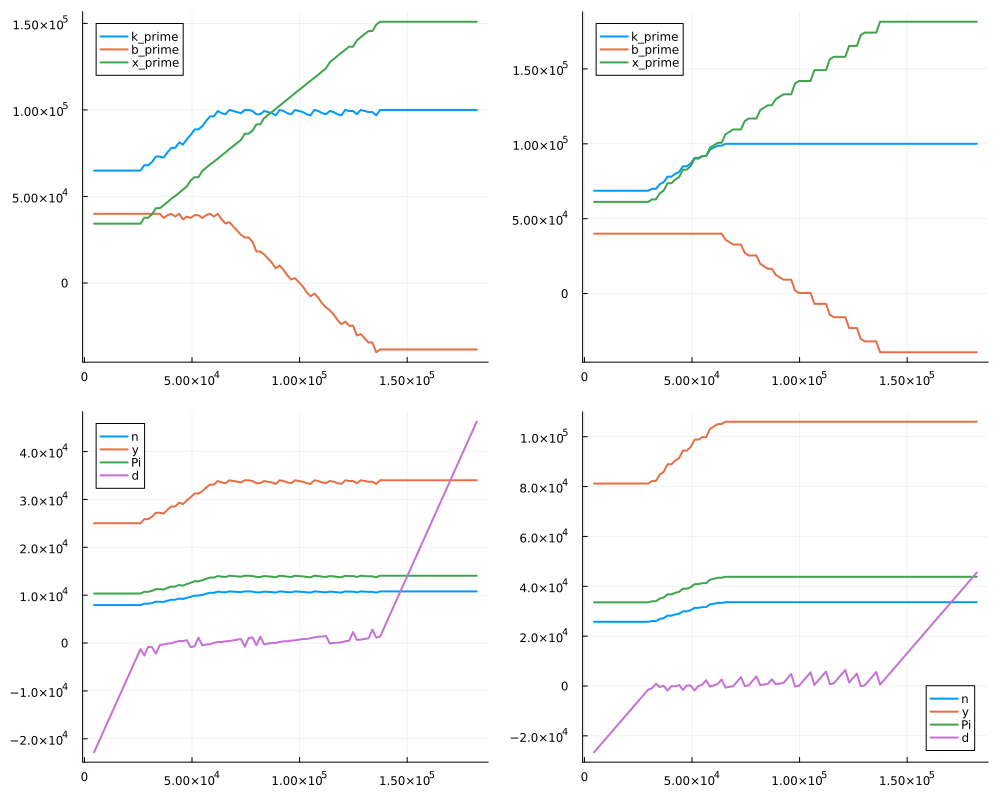
\includegraphics[width=1\textwidth]{ver2.png}
\end{figure}


\newpage
\setcounter{equation}{0}

\subsection*{Ver 3 - ABL Qs - cash on hand - AR(1) productivity}
Productivity process: AR(1) process with multiple states. Below, I plot the worst the median and the best productivity state. \vspace{3mm} \\
Labour policy: 
\begin{equation}
    n(k,\varepsilon_i) = \left( \dfrac{ \nu \varepsilon_i k^\alpha}{w} \right)^{\frac{1}{1-\nu}}
\end{equation}
Corresponding output: 
\begin{equation}
    y(k,\varepsilon_i) = \varepsilon_i k^{\alpha} \left( \dfrac{\nu \varepsilon_i k^\alpha}{w} \right)^{\frac{\nu}{1-\nu}}
\end{equation}
Corresponding profits: 
\begin{equation}
    \pi(k,\varepsilon_i) = (1-\nu) y(k,\varepsilon_i) - c
\end{equation}
Future cash on hand: 
\begin{equation}
   x' = \pi(k',\varepsilon_j')+(1-\delta)k'-b'
\end{equation}
External finance premium:
\begin{equation}
    q^{abl}(k',b')b' = \beta \left[ (1-P_\chi) b' + P_\chi \min\{b', \ \phi_k (1-\delta) k' \} \right]  
\end{equation}
Equity finance option:
\begin{equation}
    d < 0 \implies d = 1.6d
\end{equation}
Value function:
\begin{equation}
     V(x, \varepsilon_i) = \max_{k',b'}  \left( x - k' +  q(k',b',\varepsilon) b' +
            \beta (1-P_\chi) \sum_{j=1}^{N_\varepsilon} g_{ij}  V(x',\varepsilon_j') \right)
\end{equation}
Here the two innovations are that interest rates are endogenous and the productivity process is more realistic. Results makes sense, although they display this jigsaw pattern in certain regions and calibrations. \textbf{Weirdly, the model breaks down when grids are defined logarithmically.} Firms very quickly converge to their desired level of capital, even if they are cash-poor - that is because $q$ remains relatively large even for very indebted firms.

\begin{figure}[H]  % [h] indicates placing the image here
    \centering
    \caption{Ver3 - worst, median and best productivity states} \label{chart:CFLcdf}
    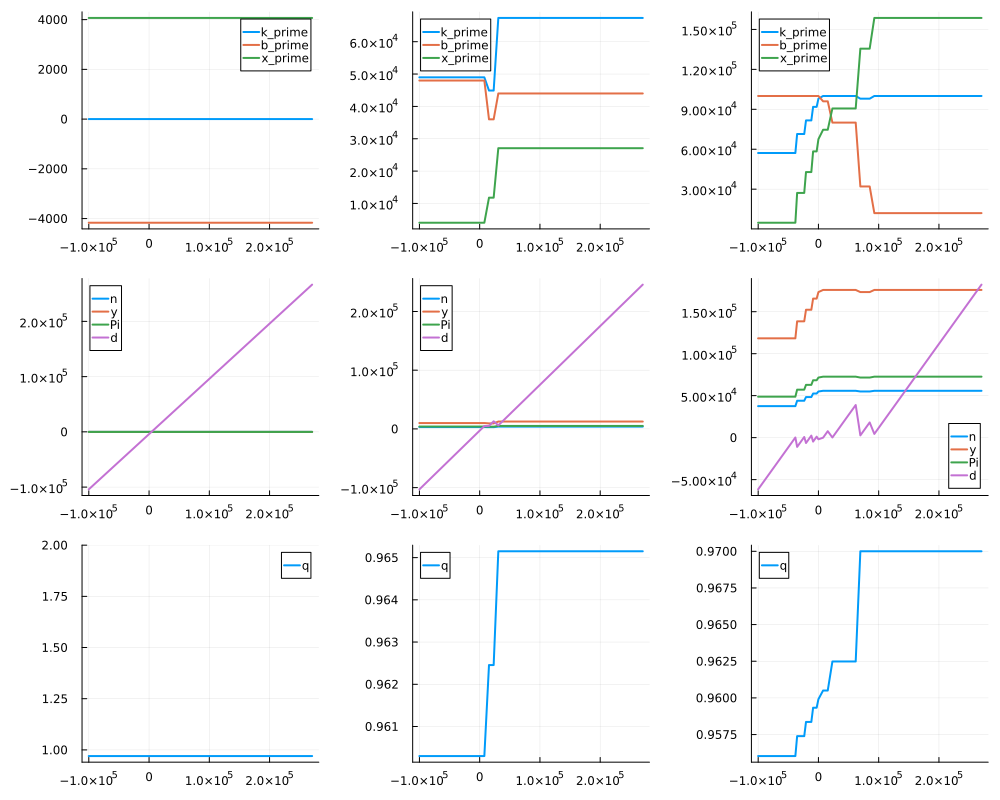
\includegraphics[width=1\textwidth]{ver3.png}
\end{figure}

\newpage

\subsection*{Ver 4.1 - Endogenous defaults, and better x-interpolation}
\textbf{Same as in Ver 3:} AR(1) productivity process, Labour policy; Corresponding output; Corresponding profits; Future cash on hand; External finance premium. \vspace{3mm} \\
Equity finance option is not necessary anymore, but I keep it with prohibitive costs. This is needed to ensure that firms have a feasible action every state.  \vspace{3mm} \\
Default decision: the firm chooses $\sigma(x, \varepsilon)$ and the corresponding $V(x, \varepsilon)$. It chooses default if $V(x,\varepsilon) \leq 0$ and $x \leq 0$ - hence the firm can fall back to limited liability and the associated value is zero. \vspace{3mm} \\
Exit decision (not implemented in this version): the firm can decide to quit without falling back to limited liability. The associated value is the cash on hand: $x$. The firm chooses this if $V(x, \varepsilon) \leq x$ and $x \geq 0$. \vspace{3mm} \\
Value functions:
\begin{equation}
    V_0 = \max \{ V_{def}, V_{exit}, V_{cont} \}
\end{equation}
where $ V_{def} = 0$, $V_{exit} = x$ and $V_{cont}$ is
\begin{equation}
     V_{cont}(x, \varepsilon_i) = \max_{k',b'}  \left( x - k' +  q(k',b',\varepsilon) b' +
            \beta (1-P_\chi) \sum_{j=1}^{N_\varepsilon} g_{ij}  V_0(x',\varepsilon_j') \right)
\end{equation}
When a firm chooses $(k',b')$ it can expect a realization of $x$, given its current $\varepsilon$. The problem is that this may not lie on the $x$ grid. In previous versions, I chose the $x_i$ on the grid that was closest to the realization of $x$. This has led to some imprecisions. Here, I make the following adjustment: if observe the two gridpoints that surround the realization of $x$. These are defined as $x_{low}$ and $x_{high}$. \vspace{3mm} \\
Then, assume that the probability of falling on these points linearly depends on the relative distance $x_{low}$ and $x_{high}$. This yields more stable results, but computing the optimal policies becomes much slower. It is probably because the Q matrix becomes more dense when with adjustment. Also, setting up Q takes longer.

\subsection*{Ver 5 - default probabilities and endogenous interest rates}

In previous iterations of the model, the interest rate was calculated on the basis of an exogenous default probability. Now you have a default decision you can update the interest rates while taking into account the endogenous default probability. I follow the following algorithm: 
\begin{enumerate}
    \item Set $q|P_{d}(exo)$, the interest rate given the exogenous default probability. Then I calculate $V(x,\varepsilon)$ given $q|P_{d}(exo)$ - which allows me to calculate the default decision for each $(x,\varepsilon)$.
    \item Now it is possible to calculate what is the probability that the firm lands on a state $(x,e)$ associated with default. This corresponds to endogenous default probability $P_d(endo)|(x,e,k',b')$ - where $P_d(endo)$ is an $n \times m$ matrix containing the default probabilities for each state-action pair.
    \item Update interest rates taking into account the endogenous default probability $q|P_{d}(exo),P_{d}(endo)$ and recalculate the optimal $k',b$ and default policies
    \item Repeat $1-3$ until the optimal policies and interest rates do not change - that is, $ (k^{i},b^{i},\chi^{i},q^{i}) = (k^{i-1},b^{i-1},\chi^{i-1},q^{i-1}) $ for each state $(x,\varepsilon)$
\end{enumerate}
\textbf{Exit decision}: In this version, I also implement endogenous exit decision. This is analogous to the default decision, with the difference that firms may keep their cash on hand if they quit voluntarily. Moreover, you need to change the value of defaulting to some small negative value ($-1000$ in this calibration). Otherwise firms always prefer to just pay all cash on hand as dividends and stay on the market for one more period on the off chance that they receive a large, positive productivity shock. 

\newpage

\section*{Summary of models up to Ver 5}

\textbf{Measure of size problem}: The cash on hand approach does not have a good measure of current size. The current cash on hand might be misleading since large debt might cancel out large capital stocks. You could do next periods' expected cash on hand, or next period's capital stock. \vspace{3mm} \\
\textbf{On interest rates}: You can rarely see default probabilities over 4\%. This is because the probability of default jumps at some point at a certain debt policy. This implies very low interest rates, which is not a good deal for the firm. Therefore in most cases, firms stop short of high levels of debt that would increase their default probabilities too much. \vspace{3mm} \\
\textbf{On debt debt policy of firms}: Here firms discount future by $\beta(1-P_\chi)$, whereas the fully secured interest rate is $\beta$. Therefore, when the firms manages to be fully secured, it prefers to hold a lot of debt and pay higher dividends, because if it default next period it might have to fall back on limited liability. This implies that even large, cash rich companies hold a lot of debt. Not a bad result, but probably not for the right reasons. \vspace{3mm} \\
\textbf{Firm growth}: Firms grow very quickly to their efficient size. A firm with no cash on hand has easy access to a lot of debt, and can grow out of cash-poorness very quickly. This might be a problem when I want to focus low wealth but productive firms. Try the reparametrization of the model - although gains here will probably be limited. Also you can also try adding a fixed cost of liquidation (paid by the lender). The advantage of this is that it can be treated purely as a calibration parameter (as opposed to default probability and resale value of capital) \vspace{3mm} \\
\textbf{Conceptualizing negative cash on hand}. How would a firm enter with negative cash on hand? You can add entry costs (usually they are needed anyways). Also you can suppose that these are distributed in a way that firms with large and negative cash on hand may enter. This is needed if you want to have cash poor but productive firms in the model. 

\subsection*{Ver 6 - Heterogeneous debt contracts}
\textbf{Same as in Ver 5:} AR(1) productivity process, Labour policy; Corresponding output; Corresponding profits; Future cash on hand; Default decision, Exit decision \vspace{3mm}  \\
Value functions:
\begin{equation}
    V_0 = \max \{ V_{def}, V_{exit}, V_{cont} \}
\end{equation}
where $ V_{def} = 0$, $V_{exit} = x$ and $V_{cont}$ is
\begin{equation}
     V_{cont}(x, \varepsilon_i) = \max_{k',b'}  \left( x - k' +  q(k',b',\varepsilon) b' +
            \beta (1-P_\chi) \sum_{j=1}^{N_\varepsilon} g_{ij}  V_0(x',\varepsilon_j') \right)
\end{equation}
External finance premium: 
\begin{equation} \label{eq:opt_tau}
    \begin{split}
        & q = \frac{\beta}{b'} \Big{[} (1-P_D)b' \ +  P_D \Big(\min \big\{ b', \ \  \gamma(k',b',\varepsilon) \left( (1-\tau') \phi_A (1-\delta) k' +\tau' \kappa \phi_A  (1-\delta) k' \right)  \\
        & \quad  +  \ (1-\gamma(k',b',\varepsilon))\left((1-\tau') \phi_A (1-\delta) k' +\tau' \left( \phi_C \E_{\varepsilon'|\varepsilon}V_2 (x', \varepsilon') - \zeta \right) \right) \big\} \Big) \Big{]} 
    \end{split}
\end{equation}
The firm has access to CF-based and asset-based debt contracts simultaneously. It chooses the optimal reliance on CF-backed debt, $\tau$ to maximize $q$. Therefore, the $\argmax$ of equation 12 describes optimal CFL reliance. The solution strategy is the same as in version 5, but now it is much more complex, hence it is also more prone to error. \textbf{It does not even converge now:}
\begin{enumerate}
    \item Set $q^0$, the starting interest rate at $\beta$ and calculate the value of the firm, $V(x,\varepsilon)$ and $k', b'$ and exit policies given  $q^0$. 
    \item Calculate the following: the probability of default $P_D$, the probability of liquidation under default $\gamma$, the liquidation value; $\phi_A (1-\delta) k'$ and the reorganization value; $V_2 (x', \varepsilon') - \zeta$ given $q^0$, for each state-action pair - meaning that all these are $n \times m$ matrices.
    \item Update interest rate, $q^1$ associated with the state-action pair, taking into account the default and liquidation probability and lenders in-default payoffs. To do this, you also need find $\tau^1$ what maximizes $q^1$ for each state-action pair. This requires an additional loop, that calculates $q^1$ given tau, and then chooses the best $\tau$.
    \item Repeat $1-3$ until the optimal policies and interest rates do not change - that is, $ (k^{i},b^{i},\chi^{i},q^{i}) = (k^{i-1},b^{i-1},\chi^{i-1},q^{i-1}) $, or at least within some tolerance value for each state $(x,\varepsilon)$.
\end{enumerate}

\subsubsection*{Ver 6 - Problems}
\textbf{The linearity of q in CFL reliance:} \\
The expected in -default payoff of the lender after the asset-based debt is: 
$$  (1-\tau') \phi_A (1-\delta) k'  $$
for CF-based debt: 
$$    \tau'\left[\gamma(k',b',\varepsilon)(\kappa \phi_A  (1-\delta) k') +  (1-\gamma(k',b',\varepsilon))\left( \phi_C \E_{\varepsilon'|\varepsilon}V_2 (x', \varepsilon') - \zeta \right) \right] $$
The borrower chooses $\tau$ to maximize the sum of these two values. Since both of them depend on $\tau$ linearly, the optimal decision on $\tau$ is 0 if the first sum is larger and 1 of the second sum is larger. Hence, this setup still cannot reproduce CFL reliance in the range of $(0,1)$. The solution would be to add a $\gamma$ that increases in $\tau$. That is, higher reliance on CF based lending increases the chance of liquidation. This is realistic if the borrower can keep whatever is leftover the default process and it gets to decide on liquidation. An example would be that a firms with a lot of unsecured debt chooses liquidation since lenders cannot enforce liquidation payments. Not too realistic but acceptable. \vspace{3mm} \\
\textbf{Adding extreme shocks}: with just the AR(1) productivity process, only a few firms end up close to cutoff values that yield non-extreme solutions. This could change if you added and extreme shock to productivity, which put firms into the best or the worst productivity bracket with some small probability. 
\newpage
Talk a bit of the non-convergence \\
Discuss future directions, talk of the misallocation approach with a particular focus on the extensive margin. And discuss the cost of small firm liquidation, is shutting the out of the market for CFL debt. 


\end{document}






 